\section{R\'ESUM\'E CONSOLID\'E PUBLIC}
\label{sec:resume}

\subsection{Résumé consolidé public en français}
\underline{Analyse d'Images d'Observation de la Terre Multi-Modales}.

Le projet MAESTRIA vise à résoudre des challenges méthodologiques relatifs à l’analyse automatique de très grands volumes d’images acquises par des plateformes d’Observation de la Terre (OT). Plus spécifiquement, MAESTRIA vise à générer des cartes d’occupation et usage des sols à l’échelle nationale, à de multiples résolutions spatiales et sémantiques, à partir d’images satellitaires multi-modales et multi-temporelles. L’objectif final est de fournir un panel large de produits d’occupation des sols qui soit exploitable autant à des échelles locales que nationales et autant pour des besoins de politiques publiques que pour la modélisation scientifique (e.g., climat, planification urbaine, suivi des cultures, détection et évaluation des changements). L’objectif de MAESTRIA est alors de développer des méthodes qui cherchent à exploiter de manière optimale les images d’OT multi-sources pour être en capacité de produire des cartes d’occupation des sols à très large échelle spatiale et avec des résolutions spatiales très variables. Le projet MAESTRIA se place dans un cadre de recherche ouverte et reproductible : codes sources et cartes générées sont mises à disposition de manière libre.

\subsubsection*{Organisation du projet}

Le processus sous-jacent est une classification supervisée dans un espace à grandes dimensions. Chaque pixel doit être assigné à une étiquette parmi un ensemble donné de classes, en utilisant (i) des caractéristiques extraites de toutes les images d'observation de la Terre disponibles d'une zone donnée et (ii) un classificateur entraîné avec des données présentant des précisions sémantiques et spatiales hétérogènes. Les problématiques posées étaient: 
\begin{itemize}
\item \textit{Comment combiner des images à très haute résolution spatiale avec des images de séries temporelles optiques à haute résolution ou des images radar} ? Cela nécessitait de développer des méthodes spécifiques pour les grandes données d'observation de la Terre afin de traiter (i) les informations complémentaires fournies par les capteurs radar et optiques, à différentes échelles spatiales et (ii) une telle quantité d'images à une large échelle spatiale.
\item \textit{Comment apprendre avec des données bruitées ?} La méthode d'apprentissage doit faire face à
du bruit dans les images ainsi que dans les données de référence et d’apprentissage. 
En outre, la taille des données de référence est généralement faible pour certaines classes, résultant en un problème de déséquilibre du point de vue du nombre de classes. La résolution d'un tel problème cherchait ainsi à réduire la dépendance à l'égard des données de référence disponibles, dont la qualité et l'accessibilité peuvent varier d'un lieu géographique à l'autre.
\item \textit{Comment obtenir des produits sémantiquement cohérents à plusieurs échelles spatiales ?} Les solutions conçues en amont devaient fournir des outils polyvalents aidant à générer des produits multiples cohérents à l'échelle nationale. Des efforts étaient nécessaires pour dériver des cartes avec une échelle spatiale et sémantique donnée à partir des classifications brutes, sans avoir recours à une nouvelle classification coûteuse pixellaire.

\end{itemize}

\subsubsection*{Résultats majeurs du projet (environ 600 caractères espaces compris)}

Les contributions majeures du projet sont doubles. Il s’agit d’une part d’une panoplie d’outils ouverts, qui facilitent la fusion et la classification multimodales d’images d’observation de la Terre puis la génération de cartes d’occupation des sols (OCS) à échelle nationale. Les problématiques de passage à l’échelle et de gestion d’images satellites multiples pour l’OCS étaient auparavant plutôt antagonistes, marquant une séparation assez nette entre une recherche opérationnelle à large échelle mais mono-capteur à une recherche plus expérimentale, plus riches en capteurs et en classes, mais non reproductible nationalement. MAESTRIA a porté la réconciliation de ces ambitions qui sont désormais nativement couplées dans beaucoup de chaînes développées et/ou opérées par des agences cartographiques ou des instituts de recherche thématiques.\\
D’autre part, le projet a participé aux évolutions de la chaîne $\iota^2$ et à son renforcement comme chaîne incontournable pour le traitement massif d’images d’OT et, entre autres, de classification d’occupation des sols dans plusieurs organismes et instituts de recherche en France.


\subsubsection*{Production scientifique et brevets depuis le début du projet}
La production scientifique s’est appuyée sur 3 thèses (dont une interrompue à mi-parcours et une non finalisée) et un ingénieur qui ont débouché, d’une part,  sur une dizaine de publications scientifiques dans des revues et conférences internationales et, d’autre part, sur des dépôts de codes et de donnés intégralement en open-source. Les développements principaux de MAESTRIA sont devenus, comme le voulait l’ambition initiale du projet, des évolutions de la chaîne \href{https://framagit.org/iota2-project/iota2}{$\iota^2$}, sur une forge publique.

\subsubsection*{Informations factuelles}

Le projet ANR MAESTRIA est un projet de recherche fondamentale coordonné par Clément Mallet (LASTIG) conjointement avec le CESBIO. Le projet a commencé en octobre 2019 et a duré 54 mois. Il a bénéficié d’une aide ANR de 568$\:$k€ pour un coût global de l’ordre de 420$\:$k€. Il a reçu le soutien du pôle de compétitivité Aerospace Valley.

\subsubsection*{Illustration}
\begin{figure}[h!]
    \centering
    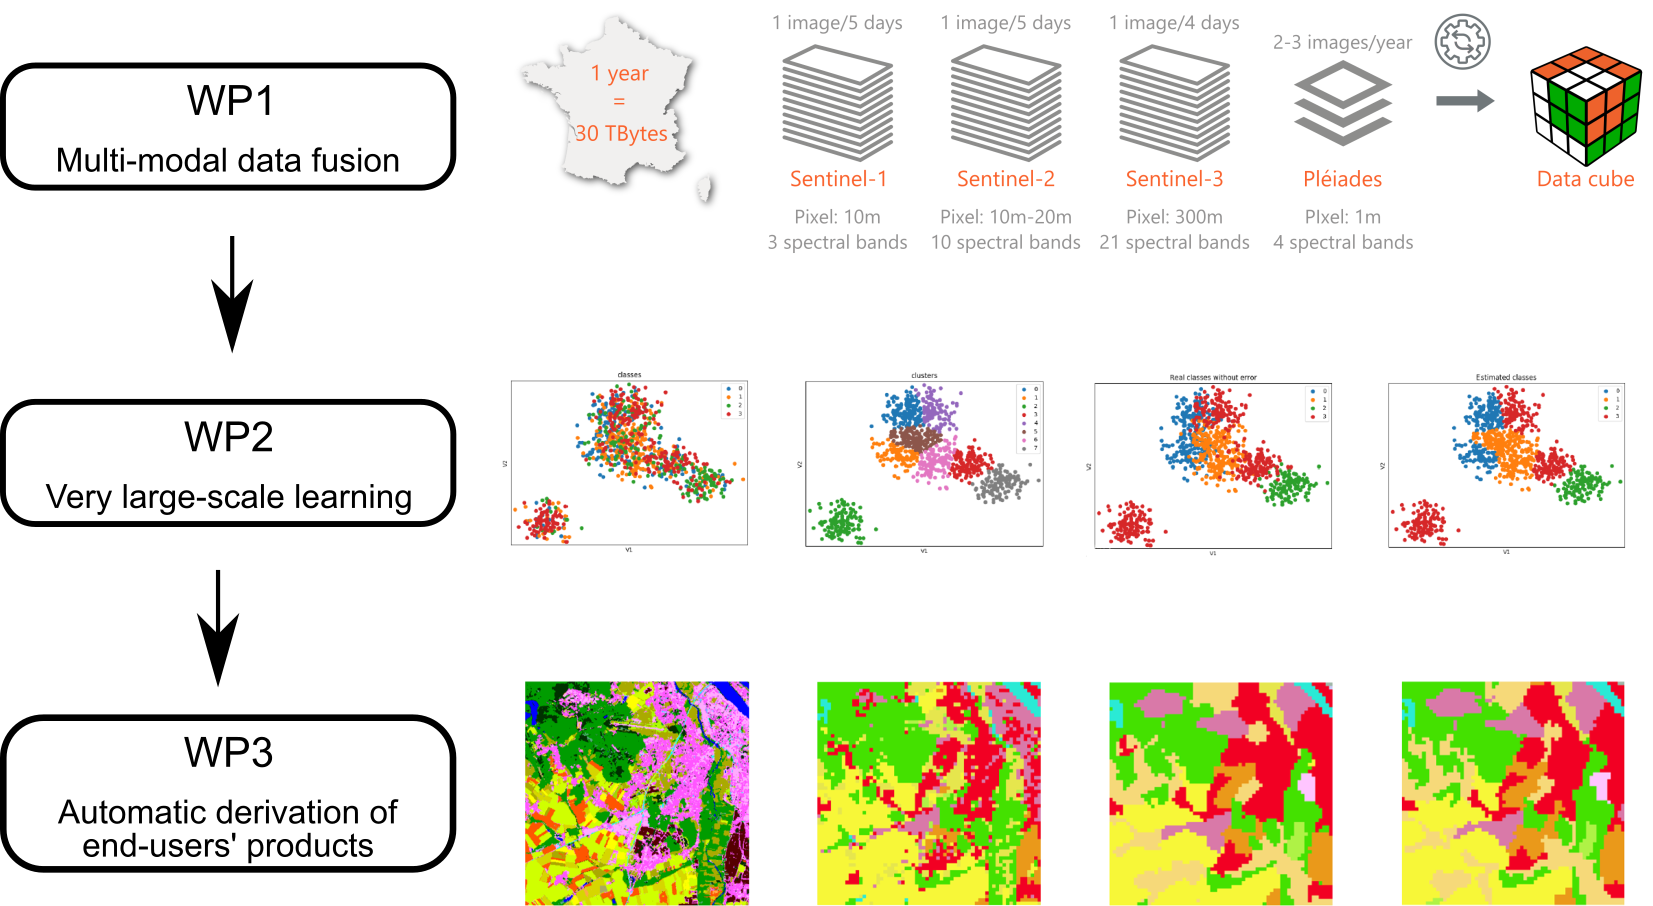
\includegraphics[width=0.9\columnwidth]{img/wp_maestria.png}
    \caption{Architecture du projet MAESTRIA. Des cartes à la demande à travers une exploitation optimale de multiples sources de données d'observation de la Terre.}
    \label{fig:enter-label}
\end{figure}






\subsection{Résumé consolidé public en anglais}

The MAESTRIA project aims to solve methodological challenges related to the automatic analysis of a very large amount of images acquired by Earth Observation (EO) platforms. More specifically, MAESTRIA aims to generate national-scale land-cover and land-use maps, at multiple spatial and semantic resolutions, from multi-modal and multi-temporal satellite images. The ultimate aim is to provide a wide range of land-cover/land-use products that can be exploited at both local and national scales, and for both public policy needs and scientific modelling (e.g., climate, urban planning, crop monitoring, change detection and monitoring). The aim of MAESTRIA is therefore to develop methods that leverage
current challenges in multisource Earth Observation image analysis
 to produce land-cover/land-use maps at very large spatial scales and with highly variable spatial resolutions. The MAESTRIA project is grounded on an open and reproducible research policy: source codes and generated maps are made freely available.